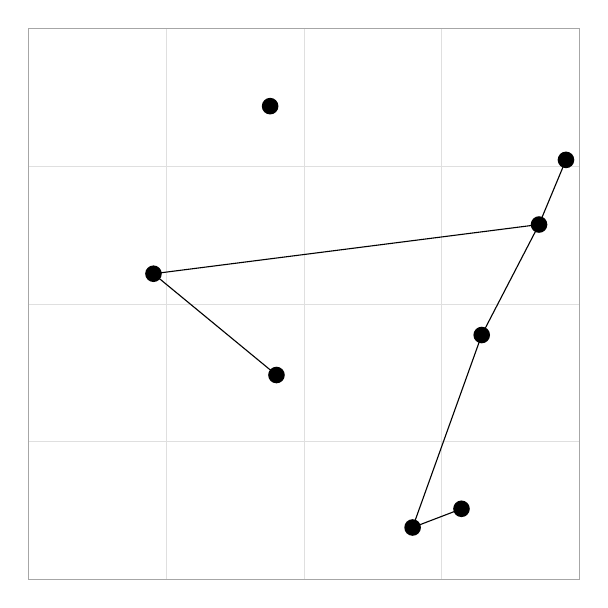
\begin{tikzpicture}[x=1.75cm, y=1.75cm]
% Generated by scripts/generate_sirg.py: seed=42, vertices=8, process=mixed-binomial(count=8), line width=0.4pt, opacity=1
% Ambient window
\draw[step=1, very thin, gray!25]
    (-2,-2) grid (2,2);
\draw[thin, gray!70]
    (-2,-2) rectangle (2,2);

% Vertices
\coordinate (v0) at (-0.24448624,1.4343917);
\coordinate (v1) at (0.78947212,-1.6232906);
\coordinate (v2) at (1.9024894,1.0445588);
\coordinate (v3) at (1.1442572,-1.4875455);
\coordinate (v4) at (-0.19845625,-0.5168079);
\coordinate (v5) at (1.70706,0.57546048);
\coordinate (v6) at (1.2910465,-0.2263432);
\coordinate (v7) at (-1.0910451,0.21833915);

% Edges
\draw[line width=0.4pt, opacity=1] (v1) -- (v3);
\draw[line width=0.4pt, opacity=1] (v1) -- (v6);
\draw[line width=0.4pt, opacity=1] (v2) -- (v5);
\draw[line width=0.4pt, opacity=1] (v4) -- (v7);
\draw[line width=0.4pt, opacity=1] (v5) -- (v6);
\draw[line width=0.4pt, opacity=1] (v5) -- (v7);

% Vertices
\foreach \v in {v0,v1,v2,v3,v4,v5,v6,v7} {
    \fill (\v) circle (3pt);
}
\end{tikzpicture}
